% !TEX root = ../double_trouble_main.tex

Past work suggests that, in a single population, we might expect the observed number of variants to grow as a power law of the number of samples \citep{Masoero2022}. \minorrevision{We discuss below how existing BNP models typically either exhibit logarithmic growth or power-law growth, each asymptotic in the number of samples, and also how power-law growth is widely recognized as desirable in BNP models.} We here rule out logarithmic growth under our model (with fixed hyperparameters) and establish results that are suggestive of power-law growth.

\paragraph{One-population review.}
\minorrevision{Before proceeding to the two-population case of interest here, we briefly support that logarithmic and power law growth are particularly common in one-population models (both for feature allocations and species sampling).
In one population, under a 3BP \internal{prior} with strictly positive discount parameter and Bernoulli likelihood, the number of features grows (asymptotically) as a power law of the number of samples \citep{Broderick2012}. Under a 3BP \internal{prior} with zero discount, the number of features grows logarithmically in the number of samples \citep{Broderick2012}. Likewise, a Dirichlet process \internal{prior} with categorical likelihood yields logarithmic growth in the number of observed species, but a Pitman-Yor process \internal{prior} exhibits power-law growth \citep[][\internal{ch.\ 3 \& 4}]{pitman1997two, Gnedin2007, pitman2006combinatorial}.}

\minorrevision{We also note that power-law growth behavior has widely been recognized as desirable in BNP models. Beyond feature models \citep{teh2009indian, lee2016bfry}, power-law growth has been extensively studied in species sampling setups, random graphs, and other domains; a necessarily incomplete list includes \citep{pitman1995exchangeable,pitman1997two,ishwaran2003generalized,pitman2006combinatorial, teh2006hierarchical, Gnedin2007, wood2009stochastic, lijoi2007controlling,teh2009indian,de2013gibbs, broderick2014combinatorial,camerlenghi2017bayesian,camerlenghi2019distribution, dolera2021bayesian,caron2012bayesian, crane2016edge, cai2016edge,archambeau2014latent}.
}

\paragraph{Two-population case.}
\minorrevision{Given these observations from the one-population case, we would like to rule out logarithmic growth (of the number of variants as a function of the number of samples) in the two-population case. A number of new challenges arise when we consider growth trends in two populations.} A first challenge is specifying how samples are collected across the two populations. In one population, there is a single way to grow the number of samples; in two populations, there are many more possibilities.
We focus on two sampling schemes 
\begin{itemize}
	\item the \emph{projection scheme}, where we sample from only one of the two populations
	\item the \emph{proportional scheme}, where we collect samples from both populations according to some fixed proportion $\propt > 0$; in particular, after $\propt$ is chosen, we have $\samplesize{2} =  \lceil\propt \samplesize{1}\rceil$.
\end{itemize}
\revision{We let $\zerovec = (0,0)$ denote a vector of zeros, and $a_\samplesizenosubscript \sim b_\samplesizenosubscript$ indicate $\lim_{\samplesizenosubscript\to\infty}a_\samplesizenosubscript/b_\samplesizenosubscript=1$. 
In this section, we establish \textit{a priori} power-law behavior for the number of new variants.
The same asymptotic behavior also holds \textit{a posteriori}, due to conjugacy of our model \citep[Section S3]{supplement}. 
\internal{For details of conjugacy and proofs}, see Section S8 in \citet{supplement}.}


\subsection{The projection scheme} \label{sec:projection_powerlaw}

First we establish power-law bounds for the expected rate of growth of the number of variants under the projection scheme. We present symmetric results for each population, so we will find it useful to introduce the notation $\notpopidx$ to indicate the population that is not $\popidx$; i.e., when $\popidx = 1$, we have $\notpopidx = 2$ and vice versa.
%%%
\begin{myProposition}[Power-law bounds under the projection scheme] 
\label{prop:power_law_proj}
	Fix hyperparameters $\mass, \conc{1}, \conc{2}, \corr{1}, \corr{2}>0$ and $\rate{1}, \rate{2} \in (0,1)$.
	Consider data drawn from the two-population model of \cref{eq:generative_model} with $\levync = \ratemeasproposed$ (\cref{eq:proposed_prior}).
	Then the number of new variants concentrates around its expectation: 
	\[
		\textrm{Fix } \samplesize{\notpopidx} = 0. \quad \news{\zerovec}{\vecsamplesize} \sim \E \news{\zerovec}{\vecsamplesize}\textrm{ a.s.\ as } \samplesize{\popidx} \to \infty.
	\]
	Moreover, there exist functions $\lowerboundproject, \upperboundproject$ that serve as respective upper and lower bounds on $\E \news{\zerovec}{\vecsamplesize}$,
	\begin{equation} 
		\label{eq:projection_bounds}
		\begin{aligned}
			&\forall \vecsamplesize, \quad \lowerboundproject(\vecsamplesize)
			\le \E \news{\zerovec}{\vecsamplesize}
			\le \upperboundproject (\vecsamplesize),
		\end{aligned}
	\end{equation}
	and that show the asymptotic behavior below.
	\paragraph{Upper bound} For either $\popidx \in \{1,2\}$ and for any $\smallpositive$ such that $0<\smallpositive\le \min\{\corr{1},\corr{2}\}$, there exists a constant $\constantupper{\popidx} > 0$ not depending on $\vecsamplesize$ such that:
	\begin{equation}
		\label{eq:power-law_projection-upperbound}
		\textrm{Fix } \samplesize{\notpopidx} = 0. \quad  \upperboundproject (\vecsamplesize)
			\sim \constantupper{\popidx} \samplesize{\popidx}^{\rate{\popidx}+\smallpositive} \textrm{ as } \samplesize{\popidx} \to \infty.
	\end{equation}
	\paragraph{Lower bound} Here let $\popidx$ be the population such that $\rate{\popidx} \le \rate{\notpopidx}$.
	Define $\rate{\notpopidx}' := \rate{\notpopidx}-\corr{\popidx}(\rate{\notpopidx}/\rate{\popidx}-1)$. 
	Then there exist constants $\constantlower{\popidx}, \constantlowerwithotherrate{\popidx}, \constantlowerwithrateprime{\popidx} > 0$
	not depending on $\vecsamplesize$ such that:
	\begin{equation}
	\label{eq:power-law_projection-lowerbound}
		\textrm{Fix } \samplesize{\notpopidx} = 0. \quad  \lowerboundproject(\vecsamplesize) \sim \constantlower{\popidx} \samplesize{\popidx}^{\rate{\popidx}}
				\textrm{ as } \samplesize{\popidx} \to \infty.
	\end{equation}
	and
	\begin{equation}
	\label{eq:power-law_projection-max_lowerbound}
		\textrm{Fix } \samplesize{\popidx} = 0. \quad  \lowerboundproject(\vecsamplesize)
			\sim \max\{ \constantlowerwithotherrate{\popidx} \samplesize{\notpopidx}^{\rate{\popidx}}, \constantlowerwithrateprime{\popidx}\samplesize{\notpopidx}^{\rate{\notpopidx}'} \}
				\textrm{ as } \samplesize{\notpopidx} \to \infty.
	\end{equation}
\end{myProposition}

See Section S8.1 in the Supplementary Material \citep{supplement} for the proof.
Note that, due to the maximum in \cref{eq:power-law_projection-max_lowerbound}, the lower bound will grow (asymptotically) at least as fast as 
$\samplesize{\notpopidx}^{\rate{\popidx}}$ as $\samplesize{\notpopidx} \to \infty$. It follows that the lower bound is (asymptotically) positive and diverging.

In the one-population 3BP, it is possible to establish almost sure power-law growth in the number of variants as a function of the number of samples \citep{Broderick2012, teh2009indian}. By contrast, here we are only able to provide power-law \emph{bounds} on the growth. Nonetheless our analysis does conclusively rule out logarithmic growth.

The gap between our upper and lower bounds depends on the population. If we take the population with lower rate parameter ($\rate{\popidx} \le \rate{\notpopidx}$), the gap between the powers in the upper and lower bounds (\cref{eq:power-law_projection-upperbound,eq:power-law_projection-lowerbound}) can be made arbitrarily close by taking $\smallpositive$ to 0. If we take the population with higher rate parameter, we generally expect a non-trivial gap between the powers in the upper and lower bounds (\cref{eq:power-law_projection-upperbound,eq:power-law_projection-max_lowerbound}). We highlight the special case where the rate parameters are equal next.

\begin{myCorollary}
    \label{coro:projection_power-law-rate-align}
    Take the same assumptions and constants as \cref{prop:power_law_proj}. Take $\rate{1}=\rate{2}=\rate{}$. Let $\popidx \in \{1,2\}$. Fix $\samplesize{\notpopidx} = 0$. Then
    	\[
		\constantlower{\popidx}\samplesize{\popidx}^{\rate{p}} \sim \lowerboundproject(\vecsamplesize) \le \E \news{\zerovec}{\vecsamplesize} \le \upperboundproject(\vecsamplesize) \sim \constantupper{\popidx} \samplesize{\popidx}^{\rate{p}+\smallpositive},
	\]
	where the asymptotic equivalences hold as $\samplesize{\popidx} \to \infty$.
\end{myCorollary}
\begin{proof}
   The result follows from \cref{eq:power-law_projection-upperbound,eq:power-law_projection-lowerbound}. \Cref{eq:power-law_projection-max_lowerbound} simultaneously applies -- with the roles of $\popidx$ and $\notpopidx$ switched -- and offers no contradiction.
\end{proof}

Despite the asymmetry of our PPP rate measure in \cref{eq:proposed_prior}, we do obtain symmetric roles for the rate
parameters across the two populations when $\rate{1}=\rate{2}$; this symmetry inspires our use of the name \emph{rate parameter} in analogy
to the one-population case.

We next simulate data from our model under the projection scheme, separately in each population (\cref{fig:power-law}); our simulations are compatible with power-law growth and with the bounds from our theory. For instance, when we grow population 1, we find that for larger $\samplesize{1}$ the number of variants grows roughly as a constant times $\samplesize{1}^{0.34}$. Since $\rate{1} = 0.3 < 0.6 = \rate{2}$, our bounds suggest growth between $\samplesize{1}^{0.3}$ and $\samplesize{1}^{0.3 + \smallpositive}$. We expect the small discrepancy is due to the finite sample. Similarly, when we grow population 2, we find that for larger $\samplesize{2}$, the number of variants grows roughly as a constant times $\samplesize{2}^{0.49}$. Since $\rate{2}' = 0.6 - 0.1(0.6/0.3-1) = 0.5$, our bounds suggest growth between $\samplesize{1}^{0.5}$ and $\samplesize{1}^{0.6 + \smallpositive}$. Again, we expect the small discrepancy is due to the finite sample size.


\begin{figure}[htp]
    \centering
    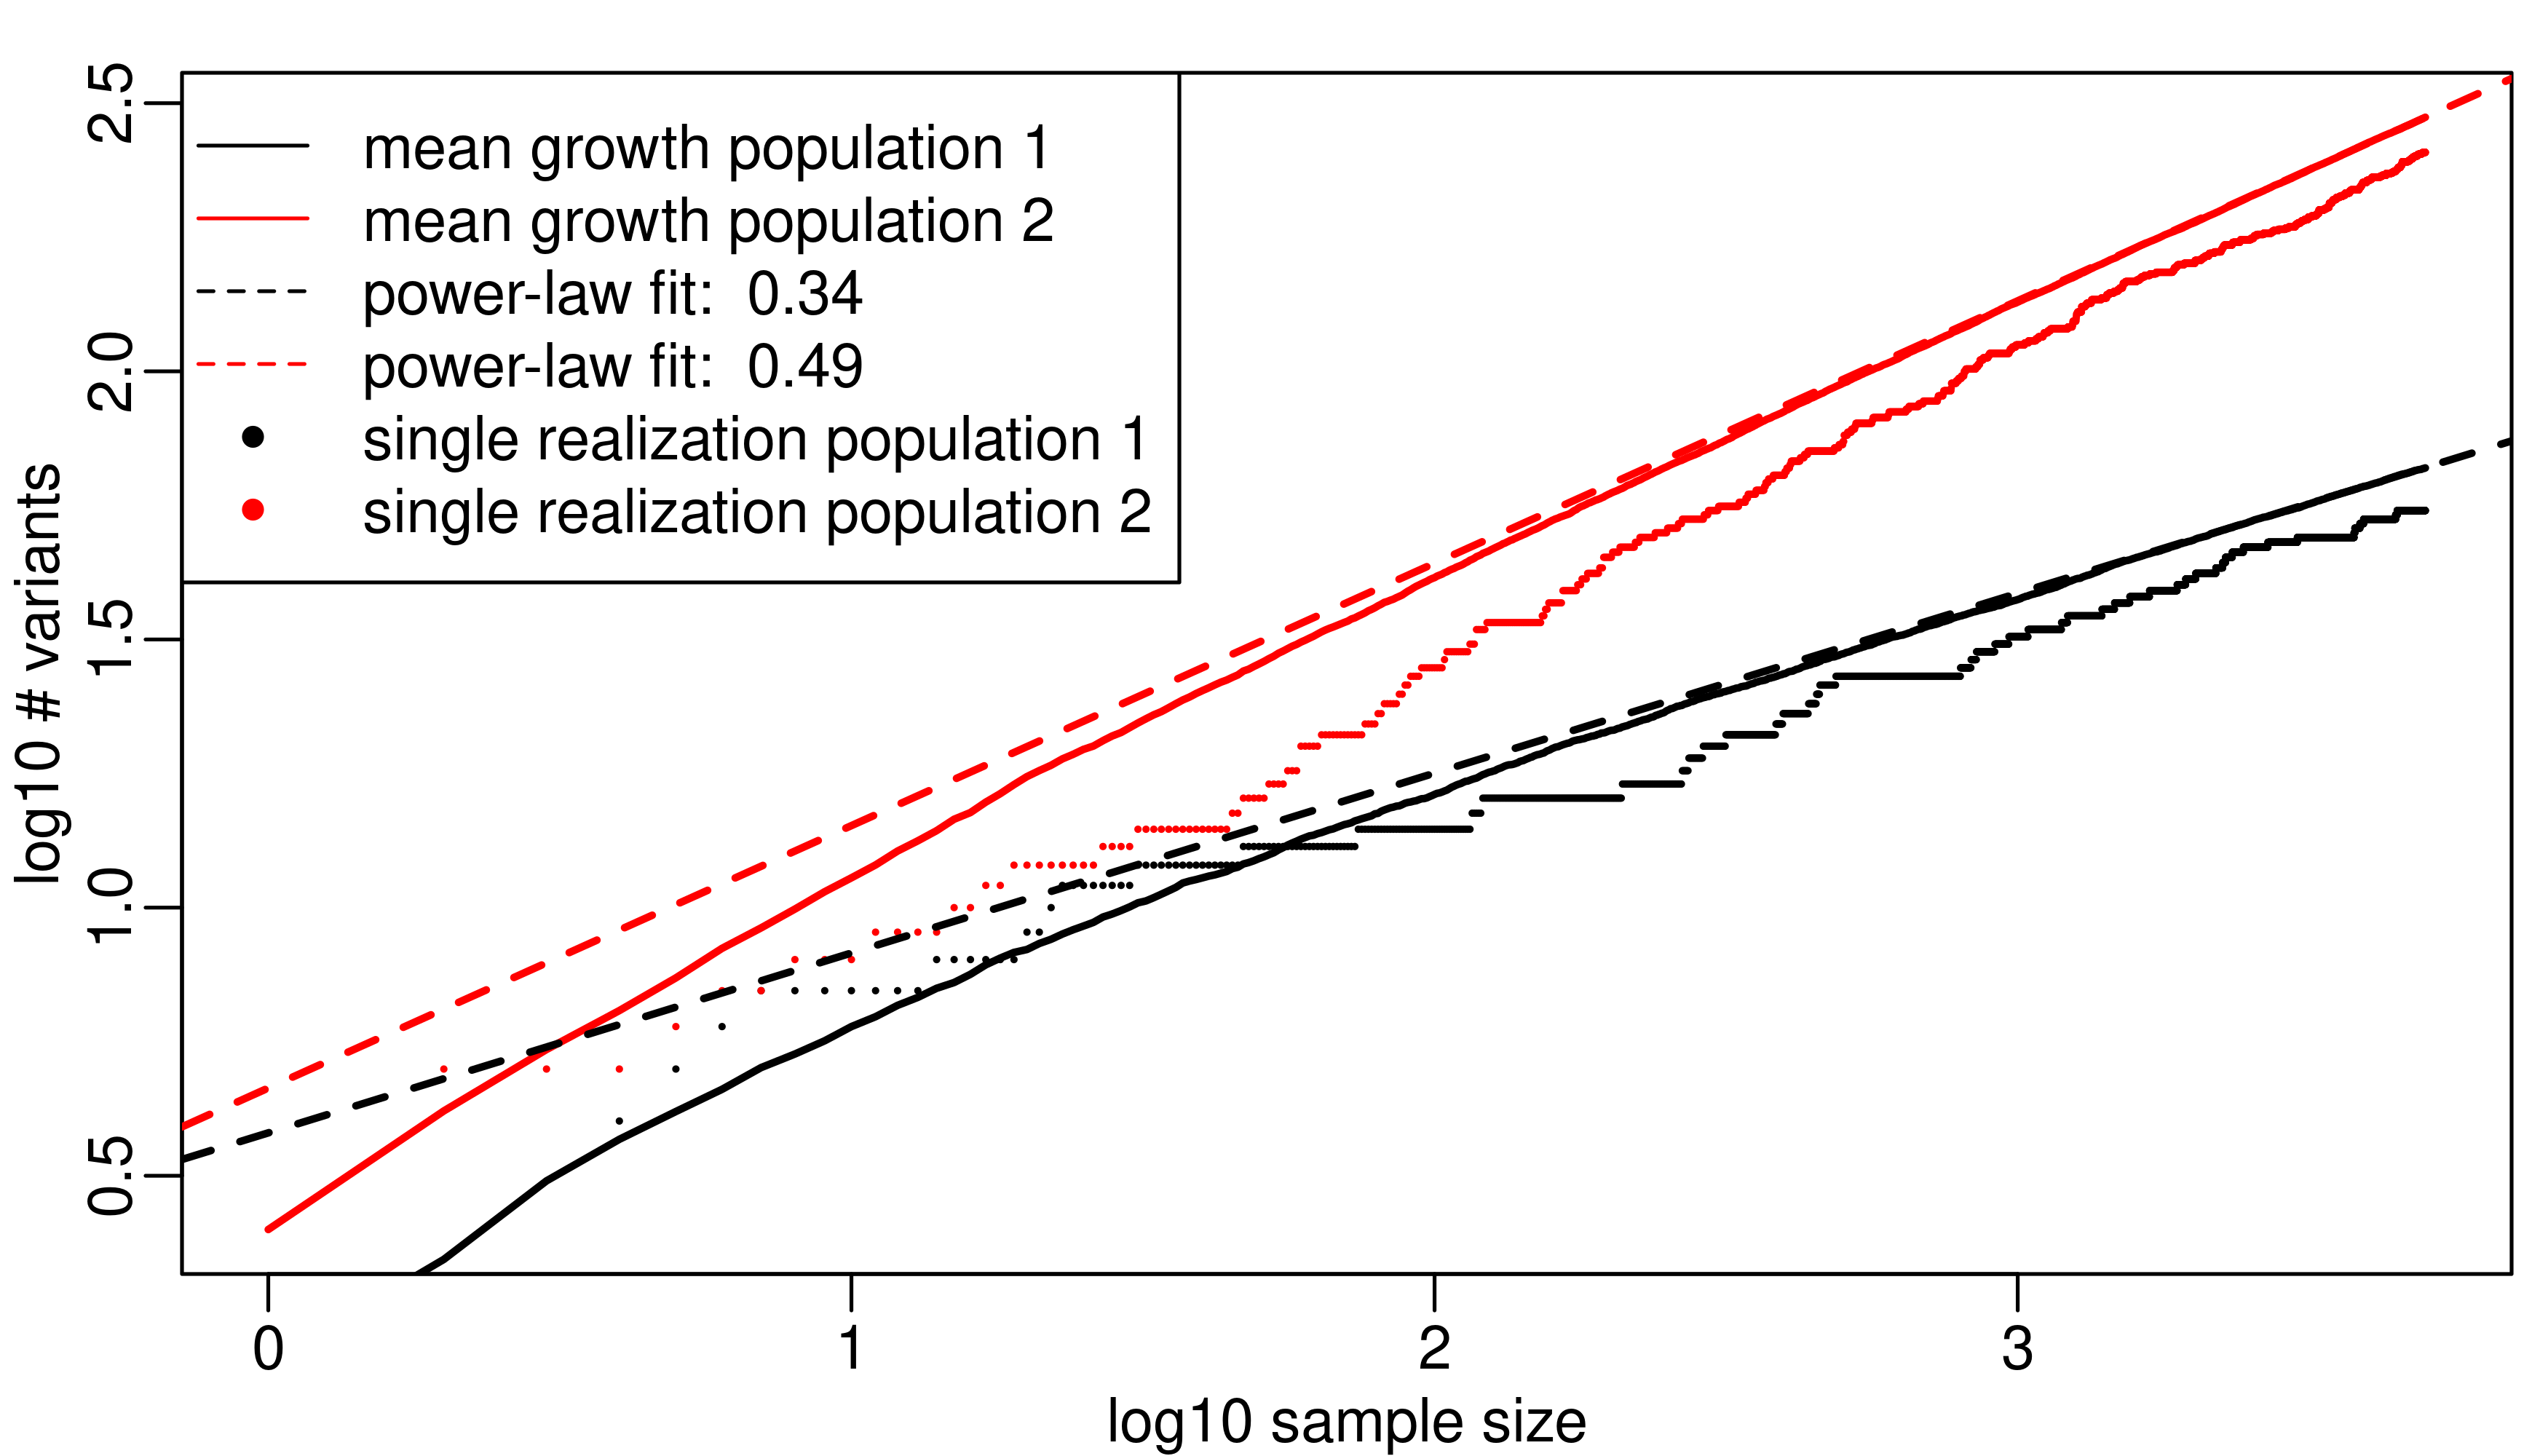
\includegraphics[width = 0.6\textwidth]{Figs/powerlaw_simu_.3_.6_.1.png}
    \caption{ \label{fig:power-law} Illustration of simulated data from our model with $\mass = 10, \rate{1}=0.3, \rate{2}=0.6, \conc{1}=\conc{2}=1, \corr{1}=\corr{2}=0.1$. Under the projection scheme, we take samples from only one population (population 1 in black and 2 in red). The observed number of variants for a given sample size is plotted as a point. To generate a solid curve, we take 100 independent realizations and plot the mean number of observed variants at a particular sample size (and interpolate between sample sizes). To plot the power-law fit, we make a linear least square fit of the log-log plot of the final third of the mean-growth curve and plot the resulting line. %note: log-log plot comes from OLS with both slope and offset parameter
	The fitted power for population 1 is 0.34 and for population 2 is 0.49.}
\end{figure}


%%%
\subsection{The proportional scheme}

We next establish power-law bounds for the expected rate of growth of the number of variants under the proportional scheme. Recall that under the projection scheme, the total number of samples was equal to the number of samples in one of the populations. Under the proportional scheme, the total number of samples will instead be $\samplesize{1} + \samplesize{2} = \lceil (1+\rho) \samplesize{1} \rceil$. We will control the asymptotics by taking $\samplesize{1} \rightarrow \infty$.
 %%%
\begin{myProposition}[Power-law bounds under the proportional scheme] 
    \label{coro:proportional}
	Take the model and hyperparameters as in \Cref{prop:power_law_proj}. Let $\popidx$ be such that $\rate{\popidx} \le \rate{\notpopidx}$, 
	
	For any $\samplesize{1}$, let $\samplesize{2} = \lceil\propt \samplesize{1}\rceil$.
	Then the number of new variants concentrates around its expectation: 
	\[
		\news{\zerovec}{\vecsamplesize} \sim \E \news{\zerovec}{\vecsamplesize}\textrm{ a.s.\ as } \samplesize{1} \to \infty.
	\]
	 Moreover,
	there exist functions $\lowerboundproport, \upperboundproport$ that serve as respective upper and lower bounds on $\E \news{\zerovec}{\vecsamplesize}$,
    \begin{equation*}
        \forall \vecsamplesize,\quad \lowerboundproport(\vecsamplesize)
        		\le \E \news{\zerovec}{\vecsamplesize}
		\le \upperboundproport(\vecsamplesize),
    \end{equation*}
	and that exhibit the asymptotic behavior we describe next. 
	Define $\rate{\notpopidx}'$ as in \Cref{prop:power_law_proj}.
	For any $\smallpositive$ such that $0<\smallpositive\le \min\{\corr{1},\corr{2}\}$, there exist constants $C,C'_{\smallpositive} > 0$ not depending on $\vecsamplesize$ such that 
    \begin{align*}
	\lowerboundproport(\vecsamplesize)
		&\sim C(\samplesize{1}+\samplesize{2})^{\max\{\rate{\popidx},\rate{\notpopidx}'\}}
			\textrm{ \ as } \samplesize{1} \rightarrow \infty \\
    	\textrm{and } \quad \upperboundproport(\vecsamplesize)
		&\sim C'_{\smallpositive}(\samplesize{1}+\samplesize{2})^{\max\{\rate{\popidx},\rate{\notpopidx}\}+\smallpositive} 
			\textrm{ \ as } \samplesize{1} \rightarrow \infty.
    \end{align*}
\end{myProposition}
See Section S8.2 of the Supplementary Material \citep{supplement} for a proof. Essentially we lower bound the total number of variants by the number seen in either population. 
We upper bound the total number of variants by the sum of variants seen in each population; this bound may be somewhat loose since some variants might be shared across the two populations, and hence double counted.  

We next present the special case where the two rate parameters are equal; in this case, the powers in the lower and upper bounds align up to an arbitrary $\smallpositive > 0$ difference.
%%%
\begin{myCorollary}
    \label{coro:proportional_power-law-rate-align}
    Take the same assumptions and constants as \cref{coro:proportional}. Take $\rate{1}=\rate{2}=\rate{}$. Then
    \begin{equation*}
        C(\samplesize{1}+\samplesize{2})^{\rate{}} \sim \lowerboundproport(\vecsamplesize)
        		\le \E \news{\zerovec}{\vecsamplesize}
		\le \upperboundproport(\vecsamplesize) \sim C'_{\smallpositive}(\samplesize{1}+\samplesize{2})^{\rate{}+\smallpositive} \textrm{\ as } \samplesize{1} \to \infty.
    \end{equation*} 
\end{myCorollary}


The result follows directly from \cref{coro:proportional} and noting that, when the rate parameters are equal, we have $\rate{\notpopidx}' = \rate{\notpopidx} = \rate{}$.

